% !TEX root = ./report.tex

\section{Molecular dynamics code}
\label{sec:mdc}

The following part is an introduction on how to use
Wentzcovitch's code to perform MD simulation. The code is
based on one of her papers (\cite{Wentzcovitch:1991ka}).

There are $4$ types of simulations in code,
denoted as \texttt{md}, \texttt{cd}, \texttt{nd}, \texttt{sd},
respectively. The first one means ``molecular dynamics'',
based on Andersen's paper, (\cite{Andersen:1980ew})
the second one means ``cell dynamics'', based on
Rahman–Parrinello approach, (\cite{Parrinello:1980kx})
the main equations are $\eqref{eq:rpeqm}$.
The third case is called ``new cell dynamics'' and is based on
$\eqref{eq:rpsdd}$ and $\eqref{eq:wenzhdd2}$,
the last one is called ``strain dynamics'' and is based on
$\eqref{eq:rpsdd}$ and $\eqref{eq:wenzhdd}$.

The simulation is done under zero temperature, as stated above.

\texttt{mxdtyp} denotes the array dimension for type of atoms,
in the input file there will be a line labeled by \texttt{(ntype)}, it
contains a scalar, i.e., number of atom types, so \texttt{mxdtyp} $=1$.

% !TEX root = ./main.tex

\subsection{Main program}

First we call \texttt{CRSTL} subroutine, see Sec. \ref{sssec:crstl} for more detail.
Second we call \texttt{INIT} subroutine, see \ref{sssec:init} for more detail.
Then we start a MD loop.
First update the current step \texttt{nzero}, and then update
accumulators \texttt{acu}, \texttt{ack} and \texttt{acp}. Then calculate
their averages by dividing \texttt{nzero}. Next we call \texttt{MOVE} subroutine,
pressure \texttt{p} is updated during this step, however \texttt{vcell} is not.
Then $P \Omega$ is calculated and a corresponding accumulator \texttt{acpv} and
average \texttt{avpv} are updated. Next update arrays like \texttt{utm} with length
\texttt{nstep} (read from input).
Then calculate the new temperature, \texttt{tnew}, by assuming equipartition
theorem $\mean{E} = \frac{ 3 }{ 2 } k_B T$, where $\mean{E}$ is
the average kinetic energy \texttt{avk}.
Then rescale the Cartesian velocity \texttt{v} and reduced velocity
\texttt{ratd}.

% Table generated by Excel2LaTeX from sheet 'Sheet1'
\begin{table}[h]
	\centering
	\caption{List of some output variables of main program.}
	\begin{tabular}{@{}rlccc@{}}
		\toprule
		\multicolumn{2}{c}{variable name}                                                 & variable symbol      & variable        & write to file                                      \\
		\midrule
		\multirow{4}[2]{*}{total}                                                         & potential energy     & $U_t$           & \texttt{utm}    & \multirow{4}[2]{*}{\texttt{e}}   \\
		                                                                                  & total kinetic energy & $E_t$           & \texttt{ekintm} &                                  \\
		                                                                                  & energy               & $\mathscr{E}_t$ & \texttt{etotm}  &                                  \\
		                                                                                  & $P \Omega$           & $P \Omega$      & \texttt{pvm}    &                                  \\
		\cmidrule{1-1}\cmidrule{4-5}    \multirow{3}[2]{*}{atomic contribution to total}  & potential energy     & $U_a$           & \texttt{utam}   & \multirow{6}[4]{*}{\texttt{eal}} \\
		                                                                                  & kinetic energy       & $E_a$           & \texttt{ekam}   &                                  \\
		                                                                                  & energy               & $\mathscr{E}_a$ & \texttt{etam}   &                                  \\
		\cmidrule{1-1}\cmidrule{4-4}    \multirow{3}[2]{*}{lattice contribution to total} & potential energy     & $U_l$           & \texttt{utlm}   &                                  \\
		                                                                                  & kinetic energy       & $E_l$           & \texttt{eklm}   &                                  \\
		                                                                                  & energy               & $\mathscr{E}_l$ & \texttt{etlm}   &                                  \\
		\cmidrule{1-1}\cmidrule{4-5}    \multirow{2}[2]{*}{average of accumulated}        & potential energy     & $\mean{U}_t$    & \texttt{avum}   & \multirow{2}[2]{*}{\texttt{ave}} \\
		                                                                                  & kinetic energy       & $\mean{E}_t$    & \texttt{avkm}   &                                  \\
		\bottomrule
	\end{tabular}
	\label{tab:lstvar}%
\end{table}%

At the end of MD loop, outputs are written to files.
Some of the output variables are listed in Tab. \ref{tab:lstvar}.
The atomic and lattice contributions could be also understood as
ionic and cell contributions, respectively. Another
important output file is \texttt{avec}, which stores lengths and angles
between primitive cell vectors for each MD step, i.e.,
$\{a, b, c\}$ and $\{\alpha, \beta, \gamma\}$,
denoted by \texttt{bmodm} and
\texttt{thetam}, respectively.
\texttt{bmodm} at each MD step
is set to lattice vectors moduli \texttt{avmod}, computed by \texttt{MOVE} subroutine.
\texttt{tv} file stores the ``instantaneous'' temperature and volume
for each MD step.


\subsection{Setup steps}

% !TEX root = ./report.tex

\subsubsection{\texttt{CRSTL} subroutine}
\label{sssec:crstl}

This subroutine does some pre-setting work before \texttt{INIT}.
An input file, named \texttt{inp}, is read to program runtime, and the flags
specified in it are parsed.
First read the $3 \times 3$ matrix \texttt{avec} from \texttt{inp} file.
If \texttt{ic} flag is \texttt{'s'},
since it is in reduced coordinates, we need to rewrite it in Cartesian
coordinates. First store the sign of each entry, then do some transformation according to
the corresponding \texttt{iop} matrix entry. The
rules are
\begin{equation}\label{eq:crstltrans}
	h(i, j) = \sign \big( h(i, j) \big) \times a_0 \times n(j)
	\begin{cases}
		\sqrt{h(i, j)},                 & \text{\texttt{iop(i,j)} is \texttt{'s'};} \\
		h(i, j)^{1/3},                  & \text{\texttt{iop(i,j)} is \texttt{'c'};} \\
		\frac{ 1 }{ 3 } h(i, j),        & \text{\texttt{iop(i,j)} is \texttt{'t'};} \\
		\frac{ 1 }{ \sqrt{3} } h(i, j), & \text{\texttt{iop(i,j)} is \texttt{'h'},}
	\end{cases}
\end{equation}
where $n(j)$ denotes the number of primitive cells along $j$th direction.
If \texttt{ic} is \texttt{'c'}, i.e., in an intermediate run, read \texttt{avec}, \texttt{avecd}, \texttt{avec2di} from last run as
input for subsequent runs, and write them to standard output.

\begin{table}[h]
	\centering
	\caption{List of some variables in \texttt{CRSTL} subroutine.}
	\begin{tabular}{@{}lcr@{}}
		\toprule
		variable name                          & variable symbol                                 & variable       \\
		\midrule
		lattice vectors matrix                 & $h = \{ \bm{a}, \bm{b}, \bm{c} \}$              & \texttt{avec}  \\
		atomic position in reduced coordinates & $\bm{s}_i = \{\xi_i, \eta_i, \zeta_i\}$         & \texttt{rat}   \\
		atomic velocity in reduced coordinates & $\dot{ \bm{s} }_i$                              & \texttt{ratd}  \\
		number of primitive cells              & $n_i$                                           & \texttt{nsc}   \\
		lattice parameter                      & $a_0$                                           & \texttt{alatt} \\
		fictitious mass                        & $W$                                             & \texttt{cmass} \\
		external pressure                      & $P$                                             & \texttt{press} \\
		reciprocal lattice vectors matrix      & $\sigma$                                        & \texttt{sigma} \\
		metric tensor                          & $g = h \tran h$                                 & \texttt{g}     \\
		metric tensor velocity                 & $\dot{g} = \dot{ h }\tran h + h \dot{ h }\tran$ & \texttt{gd}    \\
		metric tensor inverse                  & $g^{-1}$                                        & \texttt{gm1}   \\
		\bottomrule
	\end{tabular}%
	\label{tab:crstl}%
\end{table}%

Then calculate cell volume $\Omega$, metric tensor $g$ and its inverse $g^{-1}$, which are
treated as part of the outputs of this subroutine.
In addition, read positions \texttt{rat} for each atom of each type.
If \texttt{ic} flag is \texttt{'s'},
then do similar transformation of these positions as $\eqref{eq:crstltrans}$ does;
if it is \texttt{'c'}, i.e., in an intermediate step, read
\texttt{avec}, \texttt{avecd}, \texttt{avec2di} from last run,
and write to standard output.
Then it calls \texttt{SPCEL} subroutine, build a supercell along $3$ directions. On each direction,
there are $n_i$ cells, where $n_i$ is the $i$th number given in \texttt{nsc} flag.
Then read \texttt{nstep} from input file, determine how many steps are
to be performed in the following MD loop.
At last it calls \texttt{RDPP} subroutine.


% !TEX root = report.tex

\subsubsection{\texttt{INIT} subroutine}
\label{sssec:init}

First call \texttt{RANV} subroutine,
generate some initial random positions for each atom of each type.
\texttt{ilj} is the only variable set by hand in code, if it is equal to $1$,
the code will call \texttt{FORCLJ} subroutine, else it will call \texttt{FORC}
subroutine, see \ref{sssec:forc} and \ref{sssec:forclj} for differences.

Then if \texttt{calc} flag is not set to \texttt{md} and \texttt{mm},
Rahman--Parrinello approach is conducted, see \ref{sssec:rpa} for detail.
First, \texttt{gmgd}, i.e., $g^{-1} \dot{g}$ is calculated.
Then for each atom of each type,
\texttt{rat2d}, i.e., $\ddot{\bm{s}}_i = g^{-1} \dot{g} \dot{ \bm{s} }_i$ is calculated.
Also, \texttt{pim}, i.e., $\Pi$ is calculated according to $\eqref{eq:pim&frr}$.
Then $\ddot{h}$ is calculated according to $\eqref{eq:hdd}$.

If \texttt{calc} flag is set to \texttt{nd} or \texttt{nm}
then \texttt{SIGP} is called, if it is set to \texttt{sd} or
\texttt{sm} then \texttt{SIGS} is called, see \ref{sssec:sigs&p}
for more detail.
From these $2$ subroutines we know
\begin{equation}
	\ddot{d} = \frac{ \ddot{h} }{ h_0 } = \frac{ \ddot{h} \sigma_0}{V_0},
\end{equation}
where
$\sigma_0 =
\{
\bm{b}_0 \times \bm{c}_0, \bm{c}_0 \times \bm{a}_0,
\bm{a}_0 \times \bm{b}_0
\}
= \frac{ V_0 }{ 2\pi } \{
\bm{a}^\ast_0, \bm{b}^\ast_0, \bm{c}^\ast_0
\} = \frac{ V_0 }{ \{\bm{a}_0, \bm{b}_0, \bm{c}_0 \} } = \frac{ V_0 }{ h_0 }$.
However, $\ddot{h}$ is not symmetrized here, so we need to do
strain symmetrization, $\ddot{d}_{ij} = \frac{ 1 }{ 2 }
(\ddot{d}_{ij} + \ddot{d}_{ji})$, and then solve
$\ddot{h} = \ddot{d} h_0$.

The lattice contribution to kinetic energy is
\begin{equation}\label{eq:calc}
	e_l =
	\begin{cases}
		\Tr (\dot{h}\tran \sigma \sigma\tran \dot{h}),      & \text{\texttt{calc} is \texttt{nd} or \texttt{nm};} \\
		\Tr(\dot{h}\tran \sigma_0 \sigma_0\tran \dot{ h }), & \text{\texttt{calc} is \texttt{sd} or \texttt{sm};} \\
		\Tr(\dot{h}\tran \dot{ h }),                        & \text{\texttt{calc} is \texttt{md} or \texttt{mm}.}
	\end{cases}
\end{equation}

Then it calculates initial energies.
Total kinetic energy is $E_t = \sum_{i} \frac{ 1 }{ 2 } m_i v_i^2 + \frac{ 1 }{ 2 } W e_l$,
where $W$ is the fictitious mass, and $\sum_{i} \frac{ 1 }{ 2 } m_i v_i^2$
results from \texttt{RANV} subroutine.
Total potential energy $U_{t} = \sum_{i} u_i + P \Omega$, where $P$ is the external pressure,
and $\sum_{i} u_i$ results from \texttt{FORCLJ} or \texttt{FORC} subroutine.
Total energy is $\mathscr{E}_{t} = E_t + U_{t}$.

\begin{table}[h]
	\centering
	\caption{List of some variables in \texttt{INIT} subroutine.}
	\begin{tabular}{@{}lcr@{}}
		\toprule
		variable name           & variable symbol                       & variable        \\
		\midrule
		$\Pi$ matrix            & $\Pi$                                 & \texttt{pim}    \\
		forces on basis vectors & $\ddot{h}$                            & \texttt{avec2d} \\
		pressure                & $P$                                   & \texttt{press}  \\
		                        & $d = (1 + \epsilon)\tran(1+\epsilon)$ & \texttt{d2}     \\
		\bottomrule
	\end{tabular}%
	\label{tab:init}%
\end{table}%


% !TEX root = ./report.tex

\subsubsection{\texttt{MOVE} subroutine}

Then it calculates total atomic kinetic energy by
$E_a = \frac{ 1 }{ 2 } \sum_{i=1}^{N} m_i \dot{ \bm{s} }_i \tran
g \dot{ \bm{s} }_i$ for each atom of each type,
and total atomic potential $U_a = \sum_{i} u_i$ from \texttt{FORCLJ} or \texttt{FORC}
subroutines.
When it comes to the lattice contribution, it is the same as \texttt{INIT} subroutine,
i.e., as $\eqref{eq:calc}$ shows. Then lattice contribution $U_l$, $E_l$, and
$\mathscr{E}_l$ can be calculated.

\begin{table}[h]
	\centering
	\caption{List of some variables in \texttt{MOVE} subroutine.}
	\begin{tabular}{@{}rlcc@{}}
		\toprule
		\multicolumn{2}{c}{variable name} & variable symbol & variable \\
		\midrule
		\multirow{3}[2]{*}{atomic contribution to total}                                  & potential energy & $U_a$           & \texttt{uta} \\
		                                                                                  & kinetic energy   & $E_a$           & \texttt{eka} \\
		                                                                                  & energy           & $\mathscr{E}_a$ & \texttt{eta} \\
		\cmidrule{1-1}\cmidrule{4-4}    \multirow{3}[2]{*}{lattice contribution to total} & potential energy & $U_l$           & \texttt{utl} \\
		                                                                                  & kinetic energy   & $E_l$           & \texttt{ekl} \\
		                                                                                  & energy           & $\mathscr{E}_l$ & \texttt{etl} \\
		\bottomrule
	\end{tabular}
	\label{tab:move}%
\end{table}%


% !TEX root = report.tex

\subsubsection{\texttt{RDPP} subroutine}

This subroutine reads the pair-potential file.
Here \texttt{ntype} is the number of different types of atoms.
It reads the potential of $i$th atom and $j$th atom, where $j \geq i$.
So in the code we need to do some assignments like
\begin{align}
	U_{ij}      & = U_{ji},      \\
	\bm{F}_{ij} & = \bm{F}_{ji}, 
\end{align}
where $U_{ji}$ and $\bm{F}_{ji}$ are what we read from file,
thus we can save time on IO operations.


% !TEX root = ./report.tex

\subsubsection{\texttt{RANV} subroutine}
\label{sssec:ranv}

This subroutine is dedicated for setting up Maxwell distributed random velocities
at temperature $T$. A scaling factor \texttt{vfac} is calculated based on
\begin{equation}
k_B T = \frac{ 1 }{ 2 } m v^2,
\end{equation}
where $m$ is the atomic mass, and $v$ is \texttt{vfac}.
In the latter part of this subroutine, the temperature is checked (every \texttt{ntcheck} time steps),
and the velocities of atoms are rescaled by $\overline{E} = \frac{ 3 }{ 2 } k_B T$, where $T$ is current
temperature.


\subsection{Force calculation}

% !TEX root = report.tex

\subsubsection{\texttt{FORCLJ} subroutine}
\label{sssec:forclj}

The subroutine will first calculate the Cartesian distance between 2 atoms.
It will call \texttt{ELJ} subroutine for each pair of atoms $i$ and $j$, in which
the force between these $2$ atoms in both Cartesian and reduced coordinates
are calculated, and denoted as \texttt{fo} and \texttt{fos}, respectively.
More detailedly, \texttt{ELJ} uses the Lennard--Jones scheme.

The Lennard--Jones potential has general form
\begin{equation}
	U(r) = 4\varepsilon \bigg( \Big( \frac{ \sigma }{ r } \Big) ^ {12} -
	\Big( \frac{ \sigma }{ r } \Big) ^ 6 \bigg),
\end{equation}
where $r$ is the distance between $2$ atoms, $\sigma$ and $\varepsilon$
are constants.
The force is calculated by
\begin{equation}
	\bm{F}_{ji} = \frac{ 24\varepsilon }{ \sigma } (\bm{r}_j - \bm{r}_i)
	\bigg( 2\Big( \frac{ \sigma }{ r } \Big) ^ {14} -
	\Big( \frac{ \sigma }{ r } \Big) ^ 8 \bigg),
\end{equation}
where $r = \lvert \bm{r}_j - \bm{r}_i \rvert$, or equivalently, its scalar form
\begin{equation}
	F(r) = \frac{ 24\varepsilon }{ \sigma }
	\bigg( 2\Big( \frac{ \sigma }{ r } \Big) ^ {13} -
	\Big( \frac{ \sigma }{ r } \Big) ^ 7 \bigg),
\end{equation}
which is plotted in Fig. \ref{fig:ljar}.

\begin{figure}[h]
	\centering
	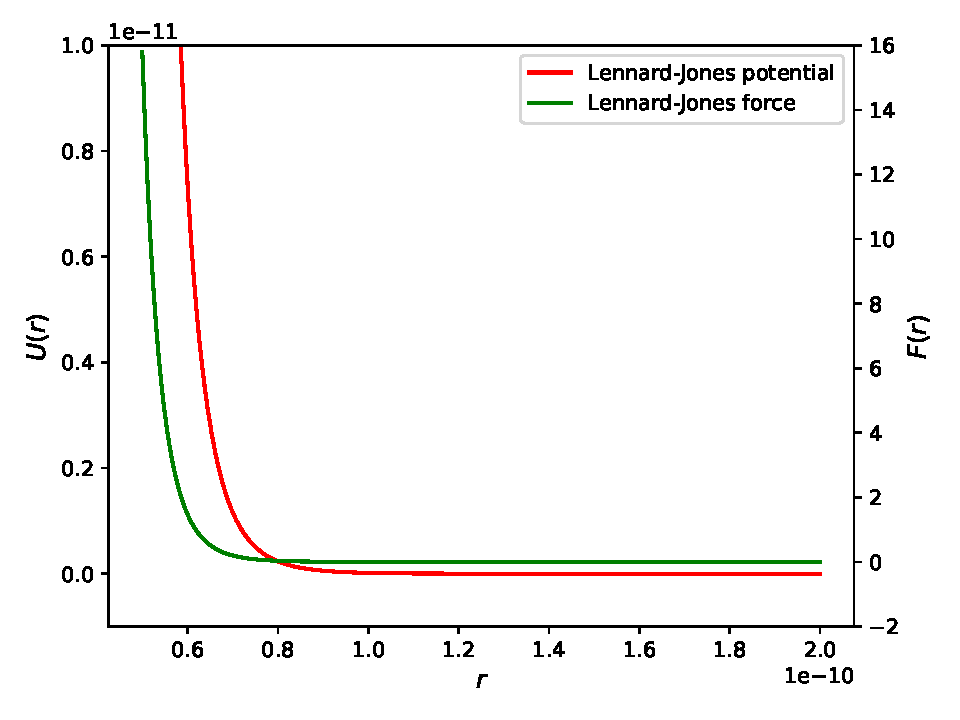
\includegraphics[width=0.5\linewidth]{lj_ar.pdf}
	\caption{Lennard--Jones potential and force for $\ce{Ar}$, as a function of
		distance between $2$ atoms, with
		$\sigma=3.405\times 10^{-10}\si{\meter}$,
		$\varepsilon = 1.654\times 10^{-21}\si{\joule}$.\cite{buffalomd}}
	\label{fig:ljar}
\end{figure}

Back to \texttt{FORCLJ} subroutine,
it considers 2 cases: particle $j$ and $i$ in the same cell and
in different cells, the first case is trivial, in the second case,
we need to add multiple times of primitive vectors and then calculate distance
$r_{ji}$, and the rest steps are the same as first case. In both cases, we do not
consider interaction out of the radius $r_{\text{cut}}$.
It appends \texttt{fo} and \texttt{fos} modified by \texttt{ELJ}
subroutine to the \texttt{f} and \texttt{fs}, respectively.


% !TEX root = report.tex

\subsubsection{\texttt{FORC} subroutine}
\label{sssec:forc}

If \texttt{FORCLJ} is used for analytical computation, then this subroutine is
used as numerical methods.
We have talked about \texttt{RDPP} subroutine before, stating that it reads
$n (n+1)$ columns of potentials and forces, denoted as \texttt{vpp} and
\texttt{fpp}, respectively.
The potentials interpolated by quadratic functions, the forces are also
calculated similar process.


% !TEX root = report.tex

\subsubsection{\texttt{UPDG} subroutine}

This part is used to update several quantities of cell during calculations.

% Table generated by Excel2LaTeX from sheet 'Sheet2'
\begin{table}[htbp]
 \centering
 \caption{List of some variables in \texttt{UPDG} subroutine.}
 \begin{tabular}{@{}llr@{}}
  \toprule
  variable name           & variable symbol                                 & variable       \\
  \midrule
  lattice vectors matrix  & $h$                                             & \texttt{avec}  \\
  lattice velocity vector & $\dot{h}$                                       & \texttt{avecd} \\
  metric tensor           & $g = h \tran h$                                 & \texttt{g}     \\
  metric tensor velocity  & $\dot{g} = \dot{ h }\tran h + h \dot{ h }\tran$ & \texttt{gd}    \\
  metric tensor inverse   & $g^{-1}$                                        & \texttt{gm1}   \\
                          & $g^{-1} \dot{g}$                                & \texttt{gmgd}  \\
  \bottomrule
 \end{tabular}%
 \label{tab:updg}%
\end{table}%


It first reads a flag \texttt{itg} to see if $\sigma$ and $V$ need to be calculated,
if it is `yes', then do the following things:
Firstly calculates $\sigma$ by the components of $h$, and then calculate the
MD cell volume by
\begin{equation}
 V = \sigma \cdot h,
\end{equation}
and then calculate $g$, $\dot{ g }$, $g^{-1}$, $g^{-1}\dot{g}$, respectively.


% !TEX root = report.tex

\subsubsection{\texttt{SIGS} and \texttt{SIGP} subroutine}
\label{sssec:sigs&p}

\texttt{SIGP} subroutine is used to calculate lattice vectors accelerations
based on `new cell dynamics', i.e., according to $\eqref{eq:rpsdd}$ and
$\eqref{eq:wenzhdd2}$; while \texttt{SIGS} is based on `strain dynamics',
i.e., $\eqref{eq:rpsdd}$ and $\eqref{eq:wenzhdd}$.
At last, the result returned is $\ddot{h}$.

In \texttt{SIGS} subroutine,
firstly calculates $f_0^{-1}$, by definition it is
\begin{equation}
 f_0^{-1} = \frac{ h_0 \tran h_0}{ V_0^2 },
\end{equation}
then set an argument \texttt{avint} to temporally store $\ddot{h}$,
and perform calculation $\ddot{h} = \ddot{h} f_0^{-1}$.
This subroutine also returns $\ddot{h}$ in the end.

In \texttt{SIGP} subroutine,
firstly calculates $f^{-1}$, by definition we know it is
\begin{equation}
 f^{-1} = \frac{ h \tran h }{ V^2 },
\end{equation}
and $e = \dot{ h }\tran \dot{ h }$, as stated above, as well as
a $3\times 3 \times 3 \times 3$ tensor
\begin{equation}
 f ' = \frac{ \partial f }{ \partial h_{ij} } = (\sigma'_{ij})\tran \sigma
 + \sigma \tran \sigma'_{ij},
\end{equation}
where $\sigma'$ is denoted as \texttt{sigmap} in code, another $3\times 3
\times 3 \times 3$ tensor.
$\dot{f}_0 = \dot{ \sigma } \tran \sigma + \sigma \tran \dot{ \sigma }$ is
also calculated.
$f^{-1} = \sum_{k, l} e_{lk} f'_{ijkl}$, and $\sigma^{-1} = h \dot{ f }$.
Then final returns $\ddot{h}$. As stated above, $h = (1 + \epsilon) h_0$,
where $h_0 = \{ \bm{a}_0, \bm{b}_0, \bm{c}_0 \}$.

